\documentclass[conference]{IEEEtran}
\IEEEoverridecommandlockouts
% The preceding line is only needed to identify funding in the first footnote. If that is unneeded, please comment it out.
%\usepackage{cite}
\usepackage{amsmath,amssymb,amsfonts}
\usepackage{algorithmic}
%\usepackage{graphicx}
\usepackage{textcomp}
\usepackage{xcolor}
\def\BibTeX{{\rm B\kern-.05em{\sc i\kern-.025em b}\kern-.08em
    T\kern-.1667em\lower.7ex\hbox{E}\kern-.125emX}}


%% Custom packages
% use biblatex with biber instead:
\usepackage[
backend=biber,
style=ieee,
sortlocale=en_US,
%natbib=true,
%url=false, 
%doi=true,
eprint=false
]{biblatex}
\addbibresource{bibliography.bib}

\usepackage{balance}
\usepackage[caption=false]{subfig}
\usepackage[toc,acronym,shortcuts]{glossaries}

%enable correct utf8 rendering
\usepackage[utf8]{inputenc}

% *** GRAPHICS RELATED PACKAGES ***
%
\usepackage{graphicx}
% Prevent figures from floating up the page
%\usepackage{flafter}
% declare the path(s) where your graphic files are
\graphicspath{{figures/pdf/}{figures/png/}}
% and their extensions so you won't have to specify these with
% every instance of \includegraphics
\DeclareGraphicsExtensions{.pdf,.jpeg,.png}

% *** DRAWING PACKAGES ***
\usepackage{tikz}
\usetikzlibrary{arrows, decorations, decorations.pathreplacing, patterns, shapes.misc}
\tikzstyle{node}=[circle,draw=black,fill=black!30,inner sep=0pt,minimum size=2.5mm]
\tikzstyle{selected}=[node,fill=black!70]
\tikzstyle{border}=[circle,draw=black,fill=black,inner sep=0pt,minimum size=1.0mm]
\tikzstyle{radio}=[circle,draw=black,dashed,pattern=dots,inner sep=0pt,minimum size=25.0mm]
\tikzstyle{mal}=[cross out,ultra thick,draw=black,inner sep=0pt,minimum size=3.0mm]
\usepackage{standalone}

\usepackage{footnotebackref}
\usepackage{enumitem}
\usepackage{bytefield}
\usepackage{subfig}
\newsavebox{\bytefieldbox}

\usepackage[disable]{todonotes}
\newcommand{\inlinetodo}[2][]{\todo[inline,caption={},#1]{#2}}
\newcommand{\todoinline}[2][]{\todo[inline,caption={},#1]{#2}}


% acronym list
\newacronym{iot}{IoT}{Internet of Things}
\newacronym{akes}{AKES}{Adaptive Key Establishment Scheme}
\newacronym{rpl}{RPL}{IPv6 Routing Protocol for Low-Power and Lossy Networks}
\newacronym{nrl}{NRL}{node revocation list}
\newacronym{coap}{CoAP}{Constrained Application Protocol}


\begin{document}

\title{Link Layer Key Revocation and Rekeying for the Adaptive Key Establishment Scheme
}

\author{\IEEEauthorblockN{Benedikt Bock}
\IEEEauthorblockA{\textit{Hasso Plattner Institute for Digital Engineering} \\
\textit{University of Potsdam, Germany}\\
benedikt.bock@student.hpi.uni-potsdam.de}
\and
\IEEEauthorblockN{Jan-Tobias Matysik}
\IEEEauthorblockA{\textit{Hasso Plattner Institute for Digital Engineering} \\
\textit{University of Potsdam, Germany}\\
jan-tobias.matysik@student.hpi.uni-potsdam.de}
}

\maketitle

\begin{abstract}
Security is a very important concern for \acl{iot} devices.
A highly specialized network stack ensures secure communication between such battery-powered IEEE 802.15.4 nodes and the internet by encrypting the messages.
This creates the necessity to manage the encryption keys using key establishment, key revocation and re-keying schemes.
The \acl{akes} introduced key establishment, but is missing a key revocation and re-keying scheme. 
So far all previously presented key revocation approaches depend in one way or another on routing messages over compromised nodes, which does not guarentee reliable key revocation.
We present a new approach that does not assume correct behavior of compromised nodes, that is efficient, provides feedback and that scales well with big networks.
We measured the performance of our implementation in a simulation environment in terms of duration and frames sent and found that it produces little overhead.
\end{abstract}

\begin{IEEEkeywords}
wireless sensor networks, AKES, Adaptive Key Establishment Scheme, key revocation, rekeying
\end{IEEEkeywords}

\section{Introduction}\label{sec:introduction}
Security and privacy is a very important aspect for \ac{iot} devices. 
As they can be deployed in a wide variety of environments: from households or smart cities to the point of sensors in the wild \cite{DanielWerner}, they often run on battery and have very narrow requirements on security algorithms and implementations. 
Nevertheless they often have access to personal informations that need to be protected against theft. 
Contiki-ng\footnote{\url{http://contiki-ng.org}} is a spin-off project of contiki\footnote{\url{http://contiki-os.org}} which itself is an open source operating system for the \acl{iot} that aims at connecting low-power microcontrollers to the \ac{iot}.
It focuses on reliable and secure, standard-based IPv6 communication.
The network stack used by contiki-ng consists of well suited protocols specialized for requirements of \ac{iot} devices. 

The \ac{akes} \cite{krentz2018denial} is one of them.
It establishes sessions keys in a denial-of-sleep-resilient way between 2 nodes which are then used to encrypt traffic on link layer level symmetrically.
A full key management life cycle consists besides key establishment of key revocation and re-keying functionality.
The last two phases were missing in the initial \ac{akes} proposal.
Therefore it was not yet possible to exclude a malfunctioning or compromised node from the network once session keys have been established.

We introduce a new key revocation schema for \ac{akes}, which supports revocation of a single or multiple nodes at a time. 
The central part of our protocol is independence of the compromised node for the revocation process to complete as well as being independent of \ac{rpl} \cite{rfc6550} to support such a feature. 
Furthermore, there is no  need for storing additional routing data on the network nodes.
As part of our approach we introduce the concept of a base station which initiates and coordinates the revocation, gains real time feedback about the revocation's progress and enables the concurrent use of multiple border nodes for faster, more efficient and more reliable key revocation. 
Our approach compares well in terms of frames sent within the network with our baseline, but takes about twice as long.

% \begin{figure}[!t]
% 	\centering
% 	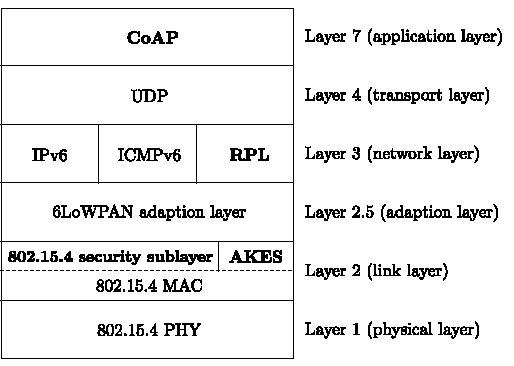
\includegraphics{network_stack}
% 	\caption{Network stack}
% 	\label{fig:network_stack}
% \end{figure}
% \inlinetodo{Do we need Fig. \ref{fig:network_stack}? If yes: Adapt Fig. \ref{fig:network_stack} to our need with bytefield.}

\section{Related Work}\label{sec:related_work}
\citeauthor{raza2016s3k} \cite{raza2016s3k} presented in 2016 an implementation based on contiki, which uses \acs{coap} unicasts to send revocation messages to each network node. 
By using unicasts they introduced the benefit of supporting a feedback mechanism. 
However, using high level protocols like the \ac{coap} arises the issue that compromised nodes are used to reach other nodes.

\citeauthor{DanielWerner} \cite{DanielWerner} published in 2018 his master thesis in which he integrates a new key revocation scheme for \ac{akes}. 
As he is using \ac{coap} unicasts like \cite{raza2016s3k}, it depends as well on the correct routing functionality of the compromised node. 
Werner furthermore presented an approach on how \ac{akes} can be extended to support blacklisting nodes using a \ac{nrl} or exclude them from further communication using re-keying.

In our approach we specify a separate trusted instance outside of the network which we call base station. 
Furthermore less energy constrained nodes get promoted to border nodes on which routing computation workload gets concentrated.
\citeauthor{jolly2003low} \cite{jolly2003low} introduced in 2003 very similar concepts of so called command nodes and gateway nodes as part of their key-management protocol for wireless sensor networks.
Nevertheless, as their network communication is based on routing messages over gateway nodes, the revocation process differs quite significantly to ours as only gateways need to be informed about the compromised node.

\citeauthor{wang2007keyrev} \cite{wang2007keyrev} presents a very energy efficient way to revoke keys for nodes by sending broadcast messages instead of unicasts. 
This approach has the drawback, that the sent messages rely on the high level routing protocol and don't avoid the compromised node. 
Moreover, their approach lacks a feedback mechanism and assumes that broadcast messages do reach every node in the network.

\section{Approach} \label{sec:approach}
%- Präsentation eures Ansatzes
%- Meistens bietet es sich an erst die grobe Idee zu vermitteln und dann erst ins Detail zu gehen
%- Auf interessante und wichtige Design-Entscheidungen eingehen
%- Modelle einsetzen
The \acl{akes} is part of the security sublayer defined in the standard IEEE 802.15.4 \cite{ieee802.15.4}.
This sublayer is part of the link layer.
During a key revocation or re-keying process the link layer topology is modified since the links between the revoked node and its neighbors are cut off or reestablished.
This means upper layer protocols (e.\,g.~\ac{rpl} on the network layer) need to adapt and are temporarily defect.
Additionally, other layers may or may not yet be aware that a node is going to be revoked and therefore should not be used during the revocation process to make sure that a compromised node is avoided for its own revocation.
We propose to use a source routing approach based on link layer messages to send revocation messages to every node. 
To explain our approach we distinguish between three different node types.
\begin{description}[style=unboxed,leftmargin=0cm]
	\item[network node]
	The network node, or just node, is every device connected to the network. 
	This node receives revocation requests and reply packages and processes them.
	\item[border node]
	In the context of \ac{akes}, every border node is a network node itself.
	However, this node type is distinguished by several features from other network nodes.
	On the one hand, it is responsible to define the route to a specific node in the network and is the communication partner to the base station.
	On the other, this node requires to be reachable directly by the base station without any other network nodes in between.
	We assume that this node is not limited in power capacity.
	%(cf.~sec.~\ref{sec:related_work})
	\item[base station]
	The base station is not necessarily part of the network itself. 
	It is used to control the network and provides an user interface. 
	In this context it is responsible to detect a compromised node and to initiate and control the revocation process of the detected node.
\end{description}

\subsection{Source Routing}\label{sec:approach:source_routing}
In our source routing approach the border node is always the initiator of a communication into the network. 
It defines the complete route to the destination.
In contrast to incremental approaches this has the advantage that nodes do not need to store any additional information and minimizes its hardware requirements.
Since we operate on the link layer we can not use IP addresses but rely on link layer addresses.
Once the border node is requested to send a revocation request to node \textit{u} it will load the route to the node and start sending a message to the first hop of the route (cf. fig.~\ref{fig:source_routing_sequence})
The receiver node will then check whether itself is already the destination node \textit{u} or just a hop on the route.
Depending on the result it will forward the package to the next hop or process the request.
Once the package was processed by node \textit{u} it will send an acknowledgement including the reversed routing information as well as all neighbors of \textit{u}.
Once this packages reaches the border node it will collect the neighbor information and allocate a route to each neighbor.
These routes can be used for further requests.
This implies that in the beginning only direct neighbors of the border node can be reached.
From that point the routing information is incrementally extended with one exception: The node \textit{m} is always ignored by the border node.
\begin{figure}[t]
	\centering
	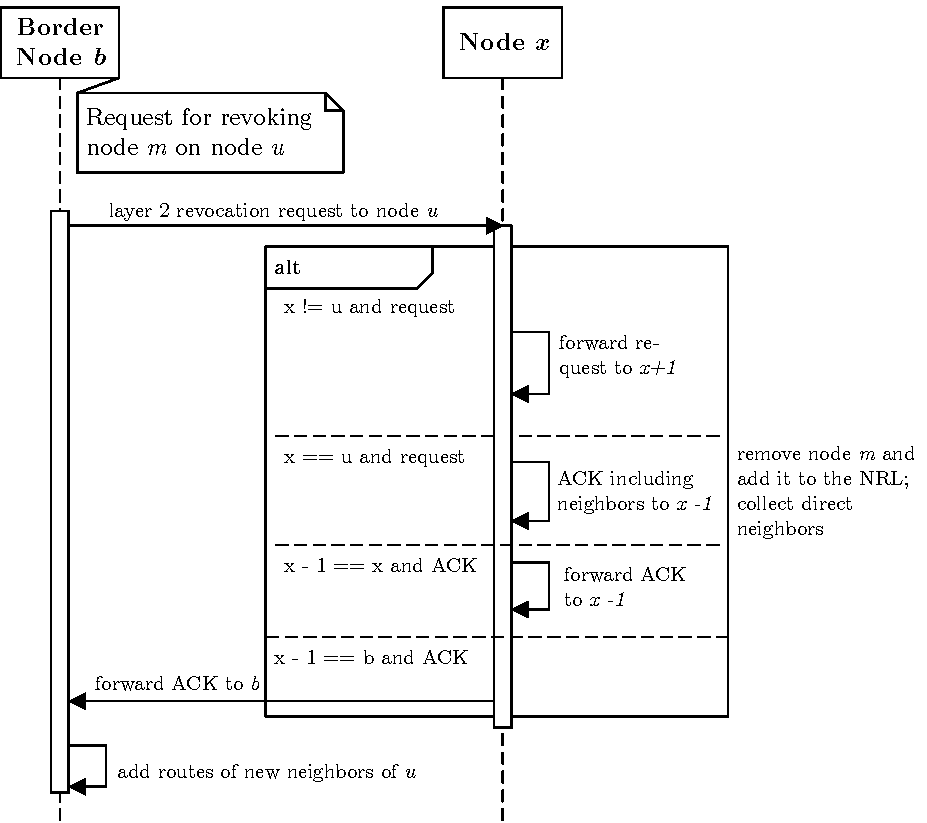
\includegraphics[width=0.49\textwidth]{source_routing_sequence}
	\caption{Source routing sequence flow for a revocation request to node \textit{u} for revoking node \textit{m}}
	\label{fig:source_routing_sequence}
\end{figure}

\subsection{Revocation Process}\label{sec:approach:revocation_process}
As mentioned previously, the base station is responsible to detect compromised nodes and to control the revocation of such nodes.
Once the station discovered a compromised node \textit{m} it will start a revocation process by requesting every border node to revoke node \textit{m} except if the border node itself is the compromised one.
If there is only one border node, it cannot be revoked.
While we assume that a border node has sufficient energy it may still be limited in other resources.
Therefore, we use the \acl{coap} \cite{rfc7252}, which is designed for low resource nodes, to communicate between base station and border node.
Every package is immediately acknowledged and processed concurrently.
Once the request is processed a border node will send a reply to the base station that contains all reached nodes from the request -- in the beginning just the border node itself.
Furthermore the reply contains a list of nodes that were discovered as new neighbors while processing the request.
These neighbors are added to a queue.
At this point a new request is sent to the border node in order to revoke node \textit{m} on the neighbors in the queue.
This happens for each border node concurrently.
The process continues until the reply has no more neighbors.
As a last step, the base station sends a termination request to the border node as soon as it did not discover new neighbors which leads to a cleared source routing cache on the border node.
If every border node is terminated the revocation process is finished.
Fig.~\ref{fig:base_station_sequence} shows this process in a sequence diagram.
Using the described process it might occur that a node remains unreached due to topology constraints (e.\,g.~node \textit{m} is the only link to the network)  or failed transmissions.
\begin{figure}[t]
	\centering
	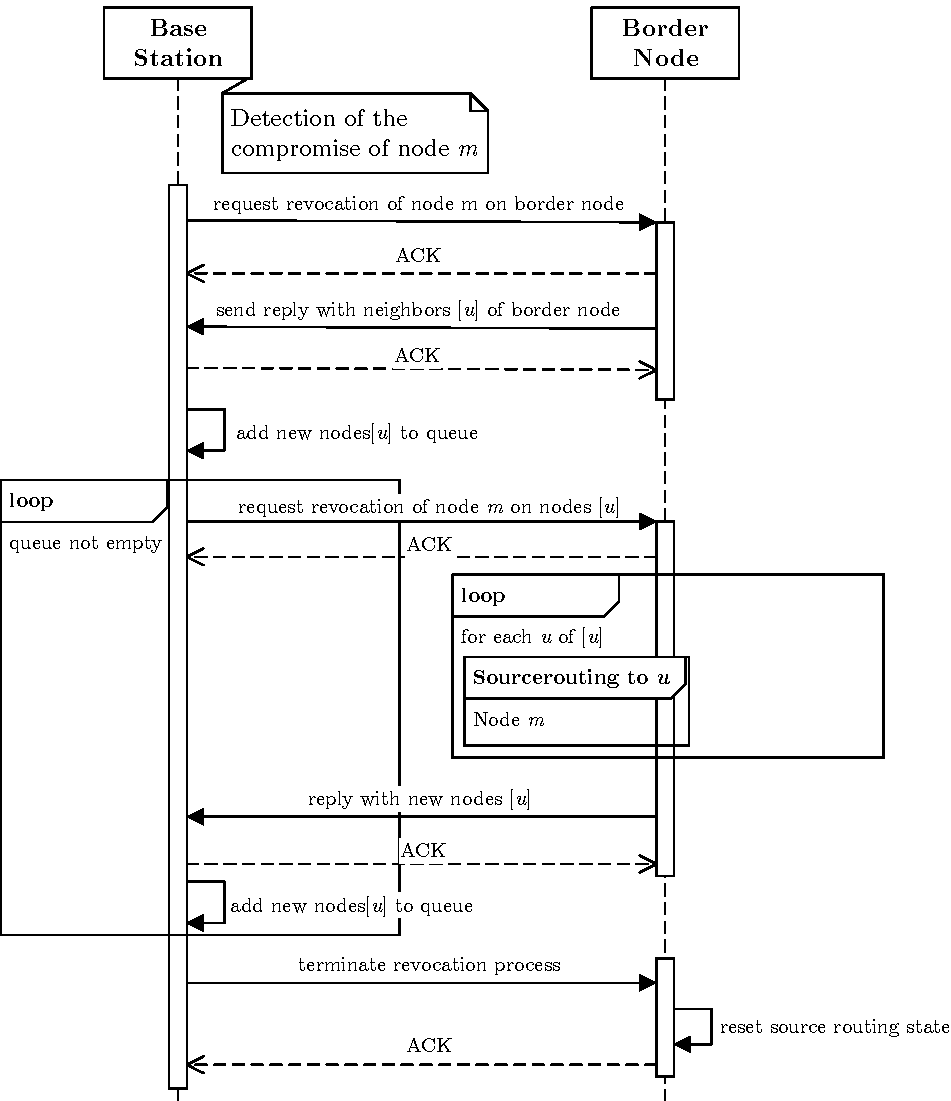
\includegraphics[width=0.49\textwidth]{base_station_sequence}
	\caption{Base station and border node communication sequence flow for a revocation of node \textit{m}}
	\label{fig:base_station_sequence}
\end{figure}

\section{Implementation}\label{sec:implementation}
%- Überlick über eure Implementierung
%- Modell der Softwarearchitektur
We implemented our approach based on contiki-ng for the network and border nodes.
It is an open-source, cross-platform operating system for \ac{iot} devices with a focus on low-power communication.
The base station is implemented with python and \textit{aiocoap}\footnote{\url{https://github.com/chrysn/aiocoap}} as \ac{coap} library.

\subsection{Message Formats}\label{sec:implementation:message_formats}
We make certain assumptions that apply to every message format introduced in this section.
Whenever a field represents a node we use the link layer address to represent it.
Therefore these fields have 8 byte, but also another identifier could be used.
We assume keys have a length of 8 byte.

In fig.~\ref{fig:coap_messages} you can see the formats of the \ac{coap} messages that are used for the communication between the base station and border nodes.
As shown in fig.~\ref{fig:coap_request} the request message consists of 5 fields.
The \textit{opts} field is a bit array of 8 bits.
Starting from the least significant bit, the first bit determines whether the message contains new keys (=1) or not (=0). 
The second bit indicates a process termination request if set to 1.
All other bits are reserved for future use and should be set to 0. 
The field \textit{node m} contains the address of the node that should be revoked on the nodes listed in the field \textit{destinations}.
In this implementation we assume that just one node gets revoked per revocation request.
In \textit{\# dsts} is defined how many \textit{destinations} and optionally \textit{new keys} are contained in the message. 
It has a range of 8 bit.
Fig.~\ref{fig:coap_reply} summarizes the content of a reply message.
The first field \textit{border id} contains the link layer address of the border node that sends the reply. 
The fields \textit{r} and \textit{n} contain the number of \textit{replies} and \textit{new nodes},
both have a range of 8 bit.
Each of the fields \textit{replies} and \textit{new nodes} contain a list of link layer addresses.
%from https://tex.stackexchange.com/questions/152907/bytefield-doesnt-work-with-subfigures
\begin{figure}[t]
	\centering
	
	\begin{lrbox}{\bytefieldbox}
		\begin{bytefield}[bitwidth=0.33em]{80}
			\bitheader{0,8,16,24,32,40,48,56,64,72,80} \\
			\bitbox{8}{opts} & \bitbox{64}{node \emph{m}} & \bitbox{8}{\# dsts} \\
			\wordbox{2}{destinations} \\
			\wordbox{2}{new keys}
		\end{bytefield}
	\end{lrbox}
	\subfloat[][request\label{fig:coap_request}]{\usebox{\bytefieldbox}}
	%%%
	
	\begin{lrbox}{\bytefieldbox}
		\begin{bytefield}[bitwidth=0.33em]{80}
			\bitheader{0,8,16,24,32,40,48,56,64,72,80} \\
			\bitbox{64}{border id} & \bitbox{8}{r} & \bitbox{8}{n} \\
			\wordbox{2}{replies} \\
			\wordbox{2}{new nodes}
		\end{bytefield}
	\end{lrbox}
	\subfloat[][reply\label{fig:coap_reply}]{\usebox{\bytefieldbox}}
	
	\caption{\ac{coap} messages}
	\label{fig:coap_messages}
\end{figure}

The messages used for source routing in the network are shown in fig.~\ref{fig:source_routing_messages}.
Our contribution focuses on the control and message distribution for revocation over re-keying processes (cf.~sec.~\ref{sec:related_work} and~\ref{sec:future_work}).
Therefore we do not provide fields for new keys.
Since all fields from the request are included in the reply, we just describe the reply.
First of all we have the \textit{hi}-field which represents the hop index. 
This value has 8 bit and is incremented with every hop.
The sender has to initialize the value to 1.
The next field \textit{hc} stands for hop count.
This is the amount of hops from sender to destination excluding the sender but including the destination.
In the following field are the addresses of each hop starting with the sender itself up to and including the destination.
This means there are $nc+1$ addresses in this field.
The next field \textit{addr revoke}, which is the last field of the request, contains the link layer address of the node \textit{m} that should be revoked.
The reply has 2 more fields compared to the request message format to accommodate the neighbors.
The amount of neighbors is depicted by the field \textit{nc} which stands for neighbor count.
It follows the list of \textit{nc} neighbor addresses.
\begin{figure}[t]
	\centering
	
	\begin{lrbox}{\bytefieldbox}
		\begin{bytefield}[bitwidth=0.41em]{64}
			\bitheader{0,8,16,24,32,40,48,56,64} \\
			\bitbox{8}{hi} & \bitbox{8}{hc} & \bitbox[tlr]{48}{} \\
			\wordbox[blr]{1}{addr sender, addr hop1,\dots, addr dst} \\
			\wordbox{1}{addr revoke}
		\end{bytefield}
	\end{lrbox}
	\subfloat[][request\label{fig:source_routing_request}]{\usebox{\bytefieldbox}}
	%%%
	
	\begin{lrbox}{\bytefieldbox}
		\begin{bytefield}[bitwidth=0.41em]{64}
			\bitheader{0,8,16,24,32,40,48,56,64} \\
			\bitbox{8}{hi} & \bitbox{8}{hc} & \bitbox[tlr]{48}{} \\
			\wordbox[blr]{1}{addr sender, addr hop1,\dots, addr dst} \\
			\wordbox{1}{addr revoke} \\
			\bitbox{8}{nc} & \bitbox[tlr]{56}{} \\
			\wordbox[blr]{1}{neighbors}
		\end{bytefield}
	\end{lrbox}
	\subfloat[][reply\label{fig:source_routing_reply}]{\usebox{\bytefieldbox}} 
	
	\caption{Source routing messages}
	\label{fig:source_routing_messages}
\end{figure}

\subsection{Network and Border Nodes}\label{sec:implementation:nodes}
These node types running on contiki-ng.
We extended the \ac{akes} implementation by several methods to receive, process and send the described messages in sec.~\ref{sec:implementation:message_formats} to get the behavior as introduced in sec.~\ref{sec:approach:source_routing}.
We did not implement the actual revocation of node~\textit{m} (cf.~sec.~\ref{sec:approach}) since we focused on how to announce revocations requests into the network.
Additionally, \citeauthor{DanielWerner} showed in \cite{DanielWerner} how the node \textit{m} can be revoked.
We discovered that our approach is rather limited in the size of the network.
With a maximum payload size of 1500 bytes and the assumption that a node has up to 4 neighbors, we can reach all nodes within a range of 17 hops.
Strategies to increase this size are discussed in sec.~\ref{sec:future_work}.

The border node additionally starts a \ac{coap} server.
With the initialization of \ac{akes} it registers a resource \textit{akes/revoke} that handles the messages of the base station.
The resource starts a seperate process to handle the request concurrently. 
The reply messages are sent from this process.
The maximum payload size of \ac{coap} packages is very limited on contiki-ng.
In order to stay in the boundaries we can only include 2 revocation requests per message sent by the base station.
This is based on the assumption that a node has a maximum of 4 neighbors.
See sec.~\ref{sec:future_work} for possible solutions.
In order to save the routing information on the border node we store every discovered node in a linked list.
Every element contains the address of the node and a reference to the parent which is the node that reported the node as neighbor at first.
This implies that there is currently only one route to every node memorized per border node.

\subsection{Base Station}\label{sec:implementation:base_station}
As described in sec.~\ref{sec:approach} the base station is not part of the network but rather a distinct device or even a virtual machine.
It consists currently of 2 modules.
First of all the \textit{NodeStore} which stores the current state of the network consisting of a list of nodes in the network and the border nodes.
The second module is the \textit{RevocationProcess}. 
This module is a singleton, since multiple concurrent revocations could lead to deadlocks in the revocation processes.
Its responsibility is to control the node revocation and to send requests to border nodes. 
It has 3 distinct caches for nodes that were already reached, nodes that need to be notified and nodes that are requested but not yet confirmed.
For the latter 2 caches each entry is a tuple of border node and node address.
This way we can try to reach a node over a different border node if the previous tries were not successful.
Once a node confirmed the revocation it gets added to the revoked cache and removed from all other caches including entries from other border nodes.
The modules use the store to check the progress.
Both modules are implemented in a thread safe manner.
There is also a \ac{coap} server started to receive the replies.
The server parses the messages and hands them over to the revocation process in a new thread.
If there are nodes that could not be reached during the process (cf. sec.~\ref{sec:approach:revocation_process}), the base station informs the user about them.

\section{Evaluation}\label{sec:evaluation}
The work of Daniel Werner \cite{DanielWerner} acts as our baseline for our evaluation. 
We aim to replicate the test scenarios presented in their work as best as possible for significant comparison. 
In the following section we will first motivate the measurements we took, explain our measurement setup and then discuss and compare the results afterwards. 
Whenever we refer to "every node in the network", we actually mean "every node but the compromised one".

The duration of a full revocation is the first characteristic we will explore. 
After a compromised node got detected it is crucial to minimize the time until this node is excluded from any further communication in order to effectively avert further harm to the integrity of the network. 
For this we measure the time, a full revocation takes from initiation by the base station till the full operation is reported back to be finished to the base station.
We omit the time it takes until each layer is updated to the new topology as it depends heavily of the protocols and configuration used.

A second important characteristic for the applicability of protocols in \ac{iot} is their impact on the total energy consumption. 
The antenna energy consumption contributes the major part to the total energy consumption of the node \cite{dunkels2007software}.
The number of active times of the antenna is therefore a good indicator for the total energy consumption. 
A single message contributes to many active times of the nodes' antennas along the route, as they forward the message to the next hop (cf. sec.~\ref{sec:approach:source_routing}). 
For transmission of a message, both antennas, the sender's as well as the receiver's, must be active. 
In conformity with Werner \cite{DanielWerner}, we refer to the time an antenna is active only for the purpose of sending, as a frame. 
The total energy consumption might then be estimated on this foundation.

For evaluation, we used the contiki simulation environment \textit{cooja}. 
We adapted the three scenarios from Werner \cite{DanielWerner} in which respectively 25, 49 or 100 nodes are arranged in a rectangular shape as shown in fig.~\ref{fig:node_network}. 
Each node is able to reach its neighbors in north, south, east and west orientation with simulated 100\% signal quality, but not diagonally.
The border node controlling the source routing is situated centered on the west side of the network. 
As our approach additionally supports the use of multiple border nodes, we created and tested a second version of each scenario, in which an additional border node is placed in the exact opposite position as the first. 
The node that got revoked was always the 3rd counted from west in the 2nd row counted from north independent of the total node count.
%\begin{figure}[!t]
%	\centering
%	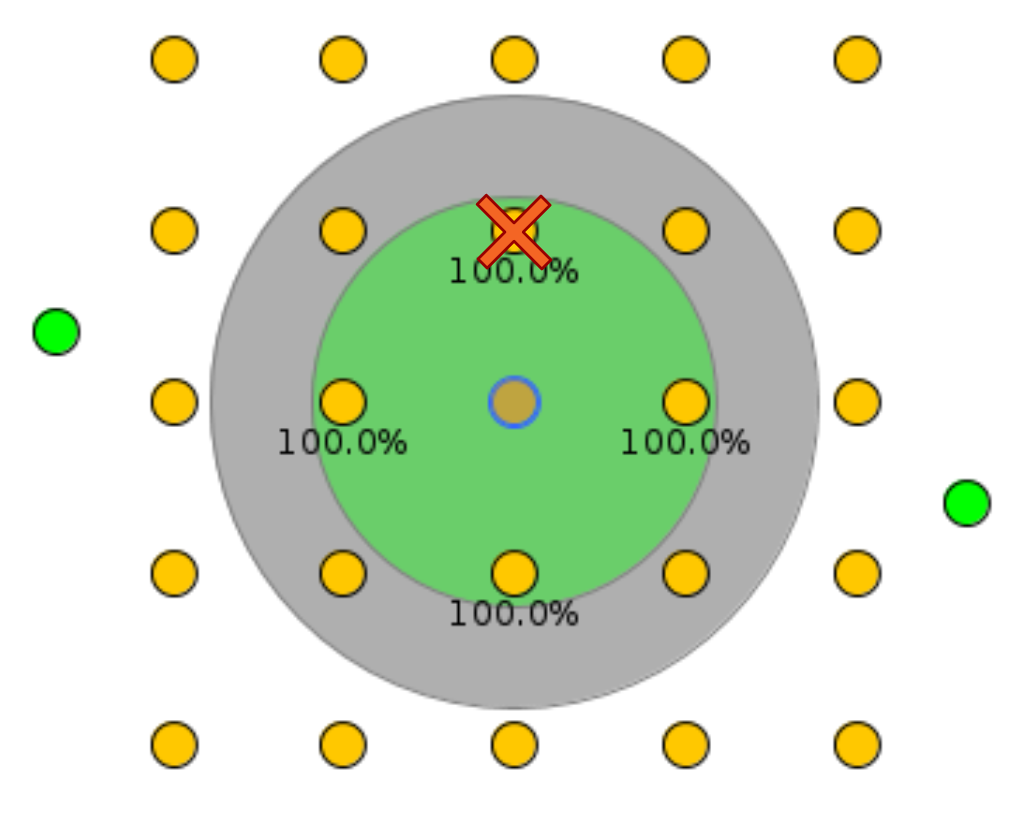
\includegraphics[width=0.2\textwidth]{node_network}
%	\caption{Node network used for simulation. [green] border nodes, [yellow] inner nodes, [cross] marks the compromised node, [green area] represents reach of wireless signal, [gray area] collision domain}
%	\label{fig:node_network}
%\end{figure}

\begin{figure}[t]
	\centering
	%\includegraphics[width=0.4\textwidth]{stage1}
	\includestandalone[width=0.3\textwidth]{figures/tikz/stage1}
	\caption{Node network used for simulation. 
		\protect\tikz{\protect\node[node] at (0,0) {}; \protect\node[border] at (0,0) {};} border nodes, 
		\protect\tikz{\protect\node[node] at (0,0) {};} network nodes, 
		\protect\tikz{\protect\node[mal,minimum size=2mm] at (0,0) {};} compromised node, 
		\protect\tikz{\protect\draw[pattern=dots, ultra thin, dashed] (0,0) rectangle (0.5,0.3);} range of wireless signal of \protect\tikz{\protect\node[selected] at (0,0) {};}}
	\label{fig:node_network}
\end{figure}

We chose to set the maximum number of destinations included in each \ac{coap} message between base station and border node to 2 (cf. sec.~\ref{sec:implementation:nodes}).
Therefore we sent half as many COAP messages as there are nodes in the network.
The implementation of the base station is written in python, hence we used the standard python "time" package for time measurement. 
The python base station process is connected to the simulation environment using unix sockets.
This might affect the transferability of the measured results onto real life node applications as artificial delays in the interprocess communication are not accounted for in the measurement.
At the beginning of each measurement we waited long enough for the nodes to boot up and most importantly for the key establishment to take place, by disabling simulation speed limits.
For representative time measurements we set the simulation speed before starting the revocation back to 100\%.
We counted the frames sent by each node in their respective message handlers in the C implementation.
Corrupted or in other ways invalid frames as well as retransmissions are not counted.

As shown in fig.~\ref{fig:duration} our approach takes about 55.5 seconds to complete a full revocation in the scenario of 100 nodes using a single border node. 
A full revocation of the baseline approach, takes only about 23 second in the 100 node scenario, which is more than twice as fast. 
The baseline uses the nullrdc MAC protocol which does not duty-cycle the nodes and therefore "decreases the overall duration of the key revocation" \cite{DanielWerner}. 
We decided against the nullrdc protocol and instead for the csma protocol for better comparability with real life applications as deactivating duty-cycling would result in much higher energy consumption.
Reducing the node count by half, does reduce the duration for a full revocation using our approach by about half as well. 
Comparing between our scenarios with one and two border nodes, the duration again gets reduced by half if a second border node is placed in an optimal position.
This shows the low overhead introduced by our implementation and the good scalability of our approach overall.
\begin{figure}[t]
	\centering
	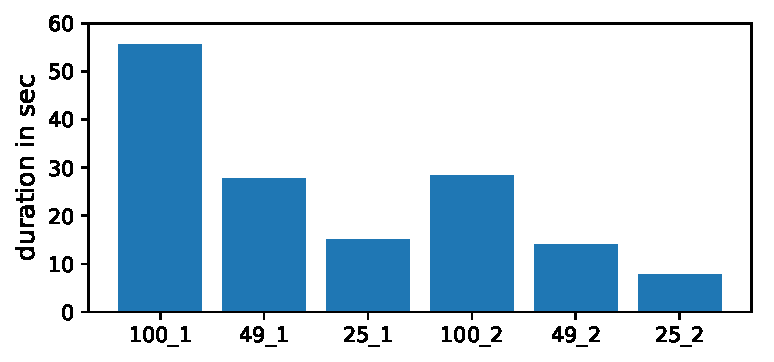
\includegraphics[width=0.4\textwidth]{durations}
	\caption{Total duration of a full revocation for node networks of the size 25, 49, 100 with one and two border nodes}
	\label{fig:duration}
\end{figure}

\begin{figure}[htbp]
	\subfloat[\label{fig:sumframes}]{%
		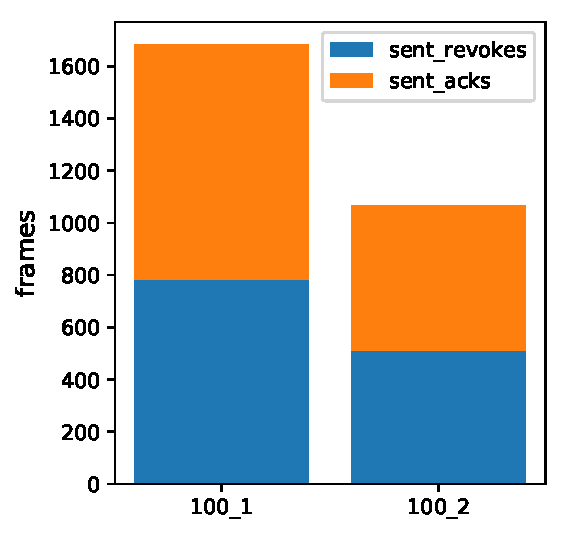
\includegraphics[width=0.2765\textwidth]{frame_sum}
	}
	\subfloat[\label{fig:frame_distribution}]{%
		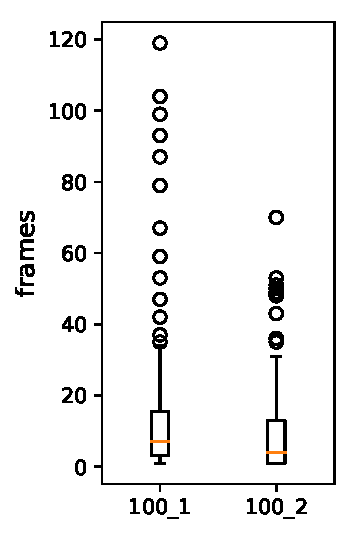
\includegraphics[width=0.175\textwidth]{frame_count_distribution}
	}
	\caption{Frames: \protect\subref{fig:sumframes} The total frames sent grouped by message type. \protect\subref{fig:frame_distribution} Distribution of the number of frames sent per node}
	\label{fig:frames}
\end{figure}

In the testing scenario with 100 nodes and a single border node, 784 revoke frames and 901 ack frames were sent.
This results in a total of 1685 sent frames.
By adding an additional border node in an optimal position, we achieved a reduction in frames sent by a number of 619 frames.
In this scenario with two border routers, exactly 513 revoke frames and 553 ack frames were sent respectively.
From an energy perspective, our approach performs well in terms of frames sent if only one border node is used, but gets way more efficient with the option of multiple border nodes.

\section{Future Work}\label{sec:future_work}

We consider the following ideas and subjects worthwhile to be investigated as part of future work.

Our approach focuses on transporting the revocation messages to each of the nodes.
Along the way a couple of attack vectors are present, especially if one assumes that other nodes may get compromised as well but were not yet detected.
If that's the case it might be possible for nodes in the middle of route to change the payload.
Therefore it is necessary to implement a way to verify at the destination node, that the content stayed unchanged.
Another attack vector might involve compromising the physically accessible border node.
If this stays undetected, the attacker could maliciously create revocation messages and send them to exclude specific nodes.
To prevent this, a verification mechanism must be in place that ensures that a secret of the trusted base station is needed for creating a valid revocation message.

Other aspects left for further work are concerning possible optimizations of our implementation. 
Issues might occure in larger networks in which long routes might cause the source routing header to reach the maximum message size. 
The first option to tackle such an issue is to implement a fragmentation solution for link layer command frames. 
This would ensure that our source routing approach can support much larger networks for the cost of adding additional message handling complexity and transmission overhead. 
Another option would be to compress header and payload to reduce the amount of data sent. 
As a frame with less data needs less time to transmit and consumes less energy, a compression of data could be very beneficial for the revocation performance overall. 
Nonetheless, it is not possible to compress arbitrarily large data without information loss. 
Hence compression is very promising but no means to support arbitrarily large node networks.
For the optimization of the \ac{coap} communication  it would be useful to consider using block-wise transfers as defined in \cite{rfc7959}.

Only after exclusion of a node by the link layer, the resulting change in the topology can be detected by all layers above it.
Especially the efficient update of the routing layer (e.\,g.~\ac{rpl}) is important for the network to become functioning again. 
\ac{rpl} incorporates an automatic process for discovering changes to the link layer node topology which triggers regularly. 
Ways to trigger this process immediately after revocation have not yet been investigated.
Although we designed our approach to be compatible with the revocation implementation presented by \citeauthor{DanielWerner} \cite{DanielWerner} we consider it worthwhile looking into the details.

\section{Conclusions}\label{sec:conclusion}
Part of a full key management cycle is key establishment, key revocation and re-keying. 
\ac{akes} introduced a key establishment scheme that is denial-of-sleep resilient, but is missing a key revocation scheme. 
Revocation of a node is very important as otherwise a compromised node could only be excluded by redeploying the whole network. 
So far all previously presented approaches depend in one way or another on routing messages over compromised nodes which cannot guarantee key revocation to work reliably. 
We presented a new approach that fulfills this requirement, that is efficient, provides feedback and that scales in a linear manner with big networks.
Our implementation produces a minimum of overhead in terms of duration and frames sent.
Our approach combined with \ac{akes}, makes up a well performing full key management cycle for \ac{iot} devices.

\balance


%\subsection{Figures and Tables}
%\paragraph{Positioning Figures and Tables} Place figures and tables at the top and 
%bottom of columns. Avoid placing them in the middle of columns. Large 
%figures and tables may span across both columns. Figure captions should be 
%below the figures; table heads should appear above the tables. Insert 
%figures and tables after they are cited in the text. Use the abbreviation 
%``Fig.~\ref{fig}'', even at the beginning of a sentence.
%
%\begin{table}[htbp]
%\caption{Table Type Styles}
%\begin{center}
%\begin{tabular}{|c|c|c|c|}
%\hline
%\textbf{Table}&\multicolumn{3}{|c|}{\textbf{Table Column Head}} \\
%\cline{2-4} 
%\textbf{Head} & \textbf{\textit{Table column subhead}}& \textbf{\textit{Subhead}}& \textbf{\textit{Subhead}} \\
%\hline
%copy& More table copy$^{\mathrm{a}}$& &  \\
%\hline
%\multicolumn{4}{l}{$^{\mathrm{a}}$Sample of a Table footnote.}
%\end{tabular}
%\label{tab1}
%\end{center}
%\end{table}

%\begin{figure}[htbp]
%\centerline{\includegraphics{fig1.png}}
%\caption{Example of a figure caption.}
%\label{fig}
%\end{figure}



\printbibliography

\end{document}
